\documentclass{article}
\usepackage[utf8]{inputenc}
\usepackage{authblk}
\usepackage{setspace}
\usepackage[margin=1.25in]{geometry}
\usepackage{graphicx}
\usepackage{xcolor}
\usepackage{float}
\graphicspath{ {./figures/} }
\usepackage{amsmath,amssymb,amsfonts}
\usepackage{booktabs}
\usepackage{natbib}
\usepackage{hyperref}
\hypersetup{colorlinks=true, linkcolor=blue, citecolor=blue, urlcolor=blue}

\title{\textbf{Trend Filtering in Crypto Markets: A Thirty-Day Time-Series Momentum Rule versus Equal-Weight Buy-and-Hold}}
\author[1]{SIQuant Research}
\affil[1]{Hypothesis $\times$ Quant}
\date{\today}
\onehalfspacing

\begin{document}
\maketitle

\begin{abstract}
\noindent \textbf{Hypothesis:} $H_0$: the Sharpe ratio of the 30-day trend rule does not exceed that of equal-weight buy-and-hold; $H_1$: it does \\
\textbf{Data:} 11 large crypto assets, 3,622 daily observations, 2016-11-25 to 2026-10-25 \\
\textbf{Method:} Long-or-cash rule on the sign of the trailing 30-day return, 10 bps costs, one-sided stationary-bootstrap test of the Sharpe difference (5,000 draws) \\
\textbf{Results:} Sharpe 1.72 versus 1.31 (difference 0.41, one-sided $p=0.0206$); maximum drawdown -62.0\% versus -86.5\%. \\
\textbf{Research decision:} \colorbox[rgb]{0.10,0.50,0.20}{\textcolor{white}{\textbf{\,ACCEPTED\,}}}
\end{abstract}

\section{Design}
The rule uses only returns up to the close of day $t-1$ to hold on day $t$ \citep{moskowitz2012time}. The look-back and the cost are fixed before the evaluation and are not tuned. An asset is included only after it has a full 30-day history.

\section{Results}
The rule is invested in 49.0\% of asset-days.

\begin{table}[H]
\centering
\caption{Net performance after 10 bps one-way costs}
\begin{tabular}{lccccc}
\toprule
Portfolio & Return & Vol & Sharpe & Max DD & Daily turnover \\
\midrule
30-day trend & 119.5\% & 54.2\% & 1.72 & -62.0\% & 7.4\% \\
Buy-and-hold & 109.4\% & 82.9\% & 1.31 & -86.5\% & 0.1\% \\
\bottomrule
\end{tabular}
\end{table}


\begin{figure}[H]
\centering
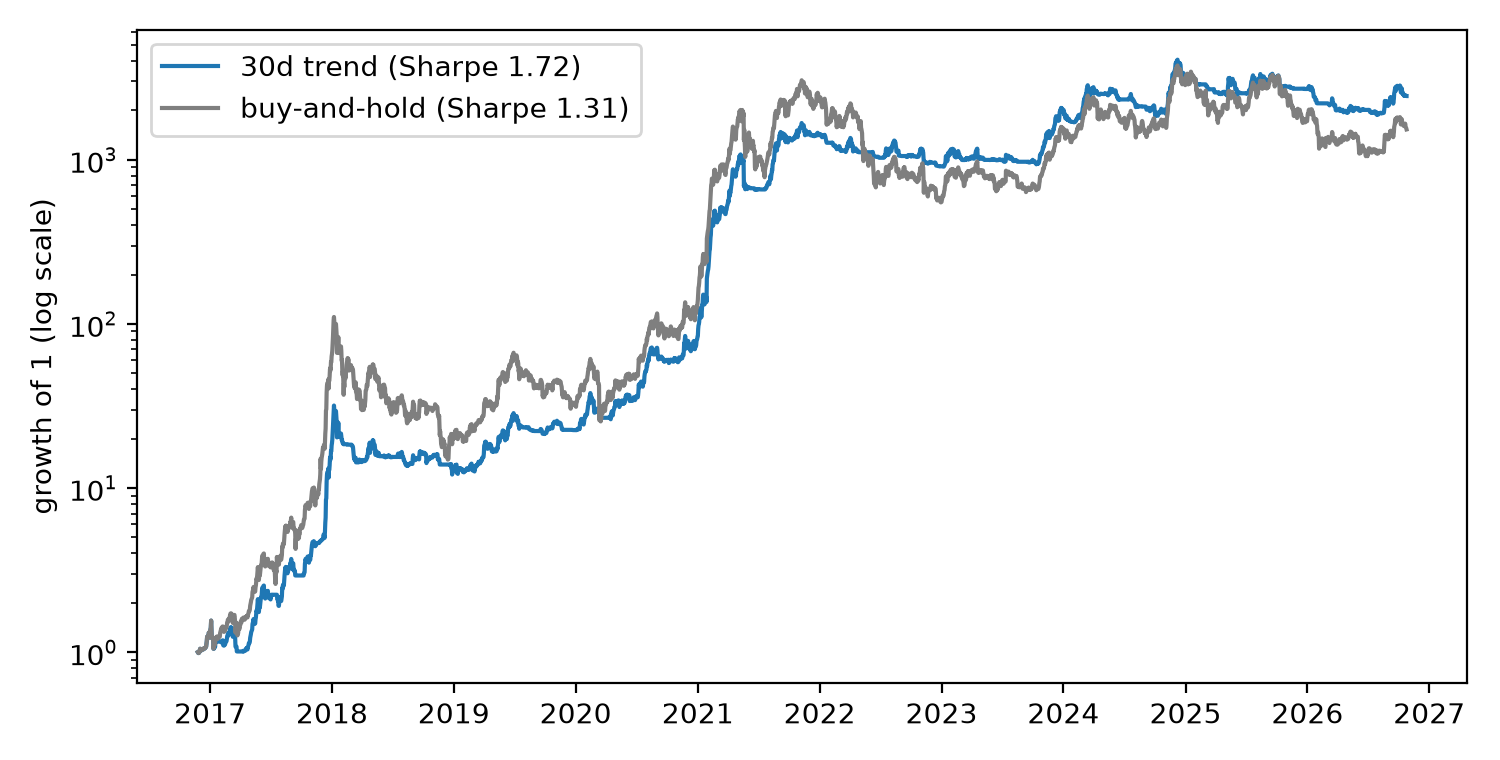
\includegraphics[width=0.8\textwidth]{fig1_trend_vs_buy_hold.png}
\caption{Growth of one unit of capital.}
\end{figure}

\section{Limitations}
The universe is today's largest assets, so there is survivorship bias that favours buy-and-hold. Returns are daily closes of Yahoo Finance quotes without spreads or funding costs. The comparison is one pre-specified rule, not a search over parameters.


\bibliographystyle{plainnat}
\bibliography{references}

\end{document}
